\phantomsection\addcontentsline{toc}{chapter}{Appendix A \quad Screenshots of the Working System}
\markboth{Appendix A}{}\expandafter\gdef\csname tp@\thepage\endcsname{}
\begingroup
\singlespacing
\begin{center}{\fontsize{14}{17}\selectfont\bfseries APPENDIX A\\ SCREENSHOTS OF THE WORKING SYSTEM}\end{center}
\vspace{-2mm}
\noindent\begin{minipage}{0.14\textwidth}
\includegraphics[width=\linewidth]{fig/demo-qr.png}\end{minipage}\hfill
\begin{minipage}{0.83\textwidth}\small The system is deployed and can be used without installation at
\mbox{\textbf{aicad-vercel.vercel.app}}. Scan the code or enter the address in a browser; the screenshots
below were captured from it.\end{minipage}

\renewcommand{\thefigure}{A.\arabic{figure}}
\setcounter{figure}{0}
\begin{figure}[htbp]
\centering
\begin{subfigure}[t]{0.49\textwidth}\centering
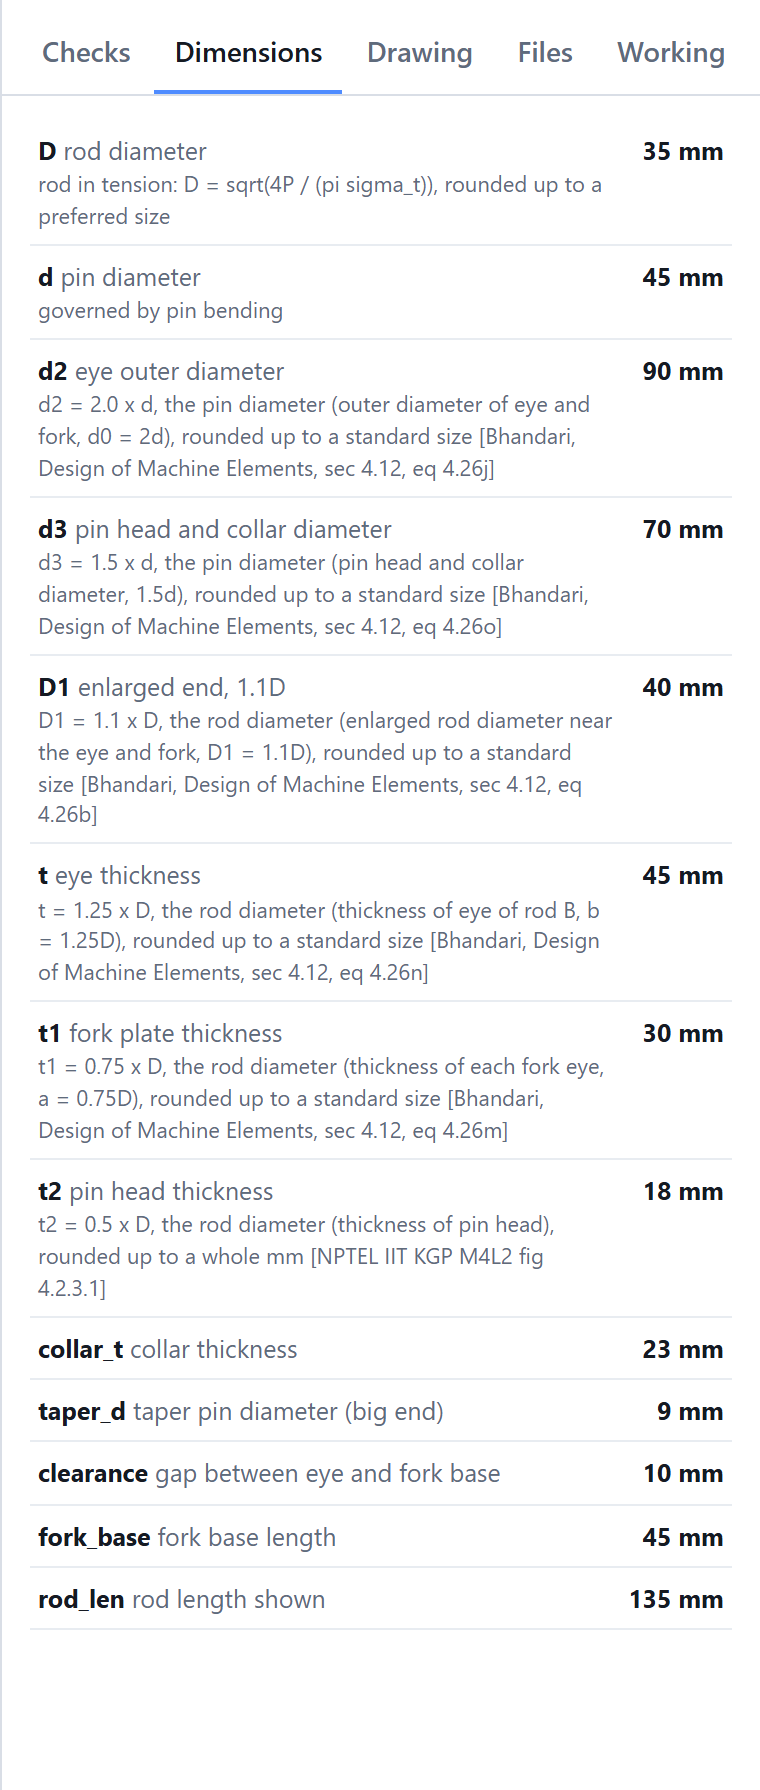
\includegraphics[height=0.32\textheight,width=\linewidth,keepaspectratio]{fig/dimensions.png}
\caption{Computed dimensions with rule and source}\end{subfigure}\hfill
\begin{subfigure}[t]{0.49\textwidth}\centering
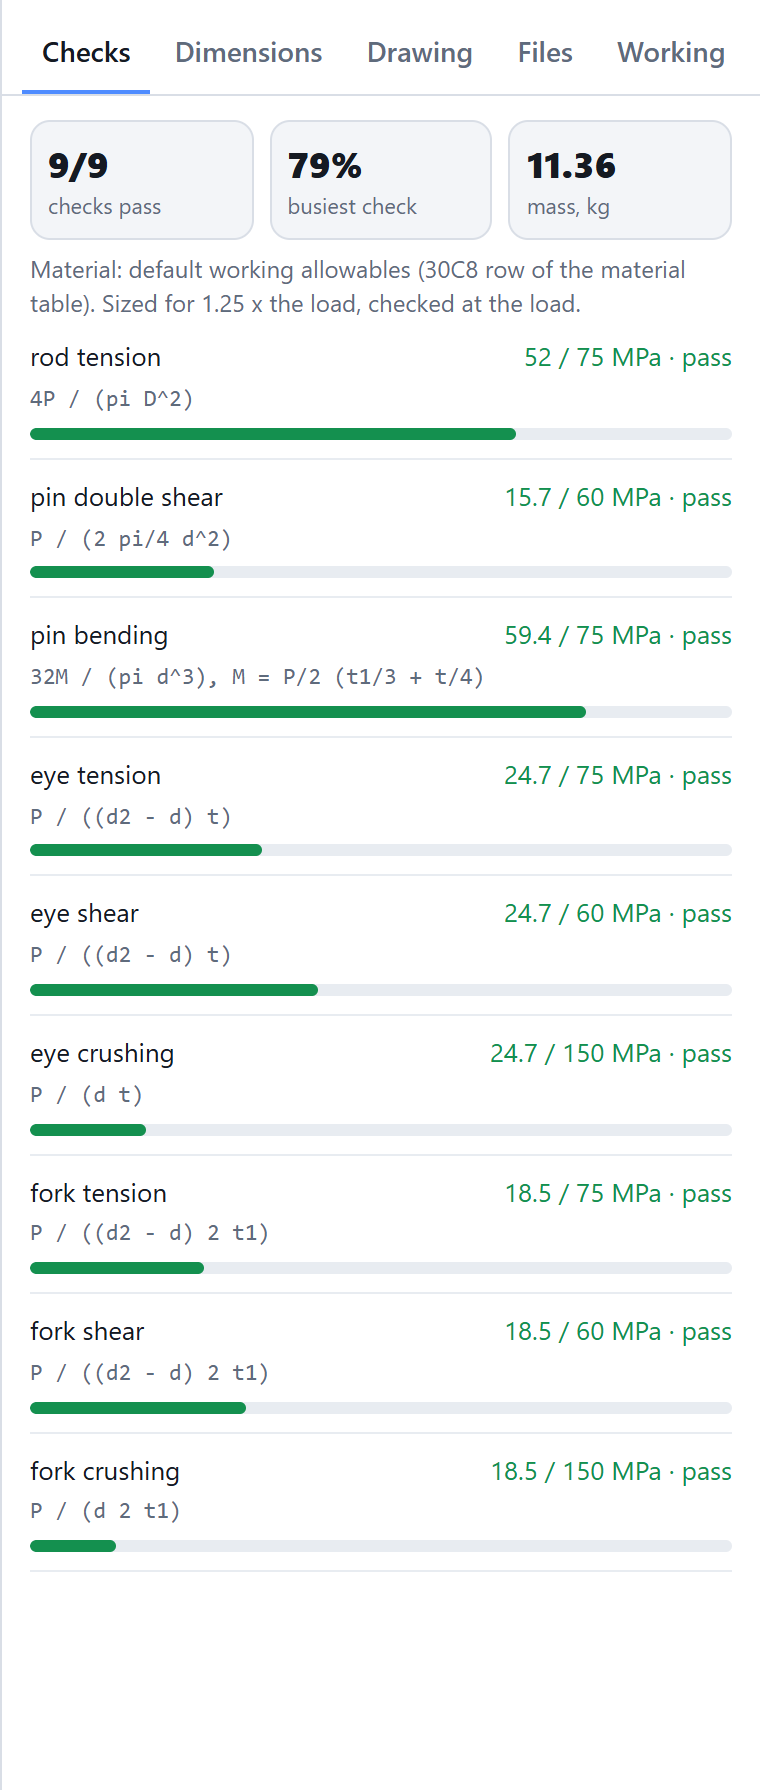
\includegraphics[height=0.32\textheight,width=\linewidth,keepaspectratio]{fig/checks.png}
\caption{Failure checks with substituted arithmetic}\end{subfigure}\\[2mm]
\begin{subfigure}[t]{0.49\textwidth}\centering
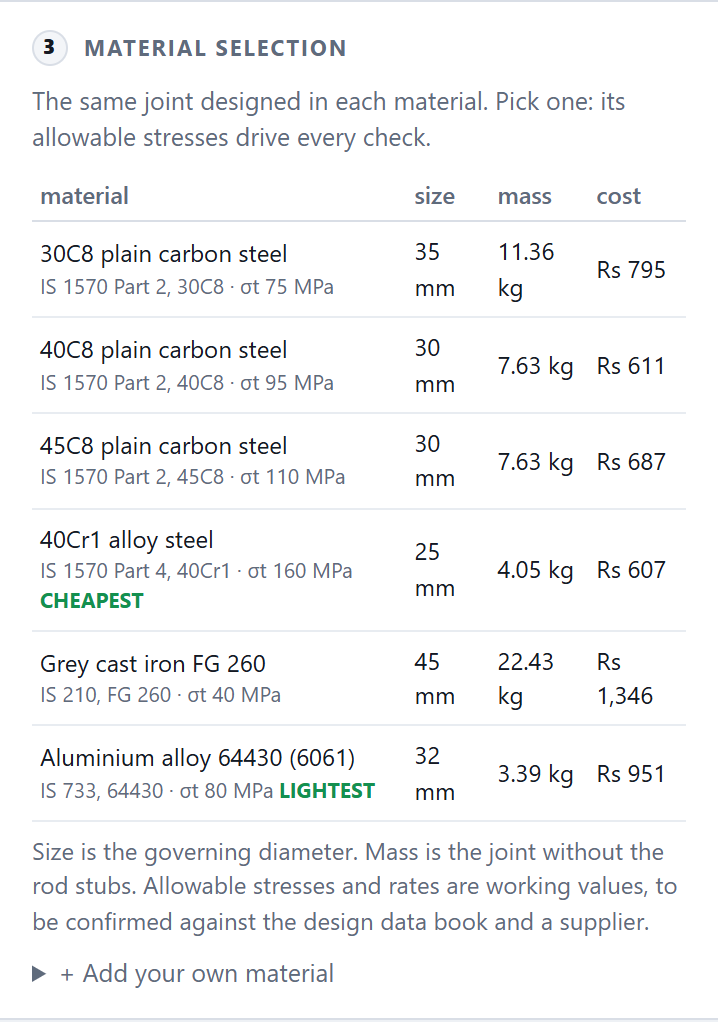
\includegraphics[height=0.32\textheight,width=\linewidth,keepaspectratio]{fig/materials.png}
\caption{Material selection}\end{subfigure}\hfill
\begin{subfigure}[t]{0.49\textwidth}\centering
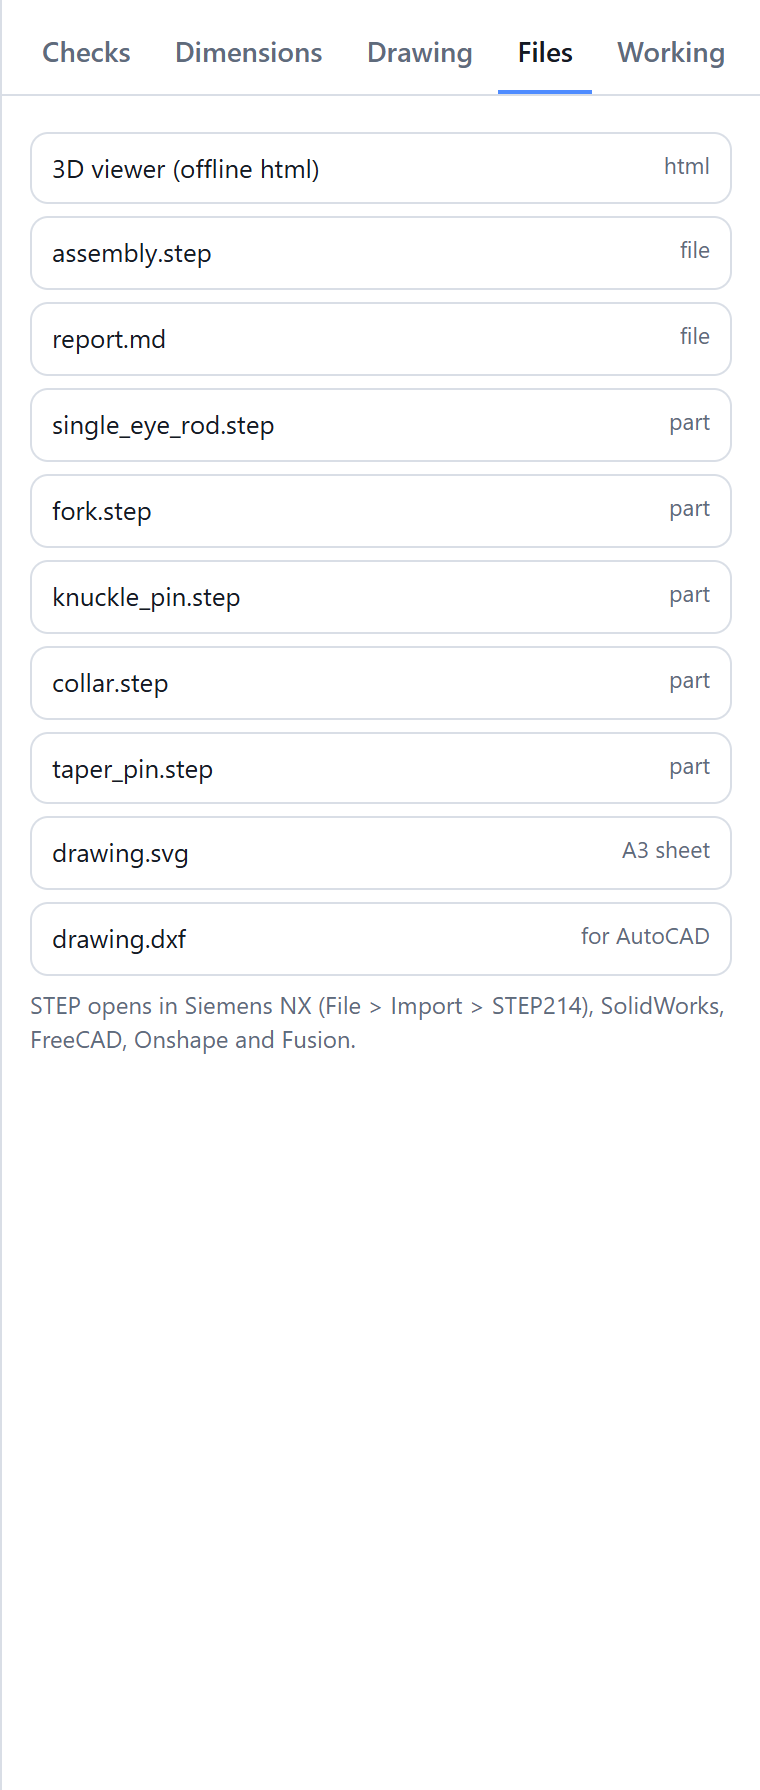
\includegraphics[height=0.32\textheight,width=\linewidth,keepaspectratio]{fig/files.png}
\caption{Files produced by a run}\end{subfigure}
\caption{Screenshots of the deployed system}\label{fig:appA}
\end{figure}
\endgroup
